\section{Sharing Data Between Clusters with \textsc{Charon}}
\label{charon}

An innovative aspect of the BiobankCloud PaaS is the capability to interconnect several PaaS deployments in a self-managed federation~\cite{ebb13}, which enables data sharing between biobanks and other BiobankCloud users.
These federations can also include public storage clouds, allowing biobanks to extrapolate the capacity of their private resources to the virtually infinite capacity of clouds without endangering the individuals' privacy.
These capabilities are implemented through a novel distributed storage system called \textsc{Charon}.

\textsc{Charon} is a cloud-backed file system capable of storing and sharing big data in a secure and reliable way using multiple cloud providers and storage repositories.
It is secure and reliable because it does not require trust on any single provider, and it supports the storage of different data sets in distinct locations to comply with required privacy premises and regulations.
Three types of data locations are supported in \textsc{Charon}: cloud-of-clouds, single (public) storage cloud, and private repository (e.g., a private cloud).
Furthermore, the private repository can be a disk in the client's machine running the \textsc{Charon} file system client, a disk in a remote machine (e.g., a private data center), or any other distributed storage system (e.g., HopsFS).

Private repositories have variable dependability and are subject to local infrastructure restrictions.
\textsc{Charon} transfers data from one private repository to another securely through encrypted channels.
The single-cloud scenario allows the controlled data sharing between two biobanks, but its dependability directly depends on a single entity -- the chosen public cloud provider.
The multi-cloud (or cloud-of-clouds) data replication is a possible location to store data, and is where \textsc{Charon} stores all its metadata securely.
It avoids having any cloud service provider as a single point of failure, operating correctly even if a fraction of the providers are unavailable or misbehave (due to bugs, intrusions, or even malicious insiders)~\cite{depsky13}.
Independently from the chosen data location, the data stored in \textsc{Charon} can be shared among mutually-trusted system users.

Figure~\ref{fig:charon} illustrates a deployment scenario where two biobanks store their data in diverse storage locations---private repositories, single public cloud providers, and a resilient cloud-of-clouds.
In this scenario, the namespace tree has six nodes: directories \texttt{d1} and \texttt{d2}, and files \texttt{A}, \texttt{B}, \texttt{C}, and \texttt{D}.
The namespace is maintained in the cloud-of-clouds, together with file \texttt{B}.
File \texttt{D}, less critical, is kept in a single public cloud.
File \texttt{A} is stored locally because it cannot leave biobank 2 (e.g., due to legal constraints).
File \texttt{C} is shared between the two sites (e.g., in the same legal framework), thus being stored in both of them.

%\vskip-8pt
\begin{figure}[ht]
 \centering
 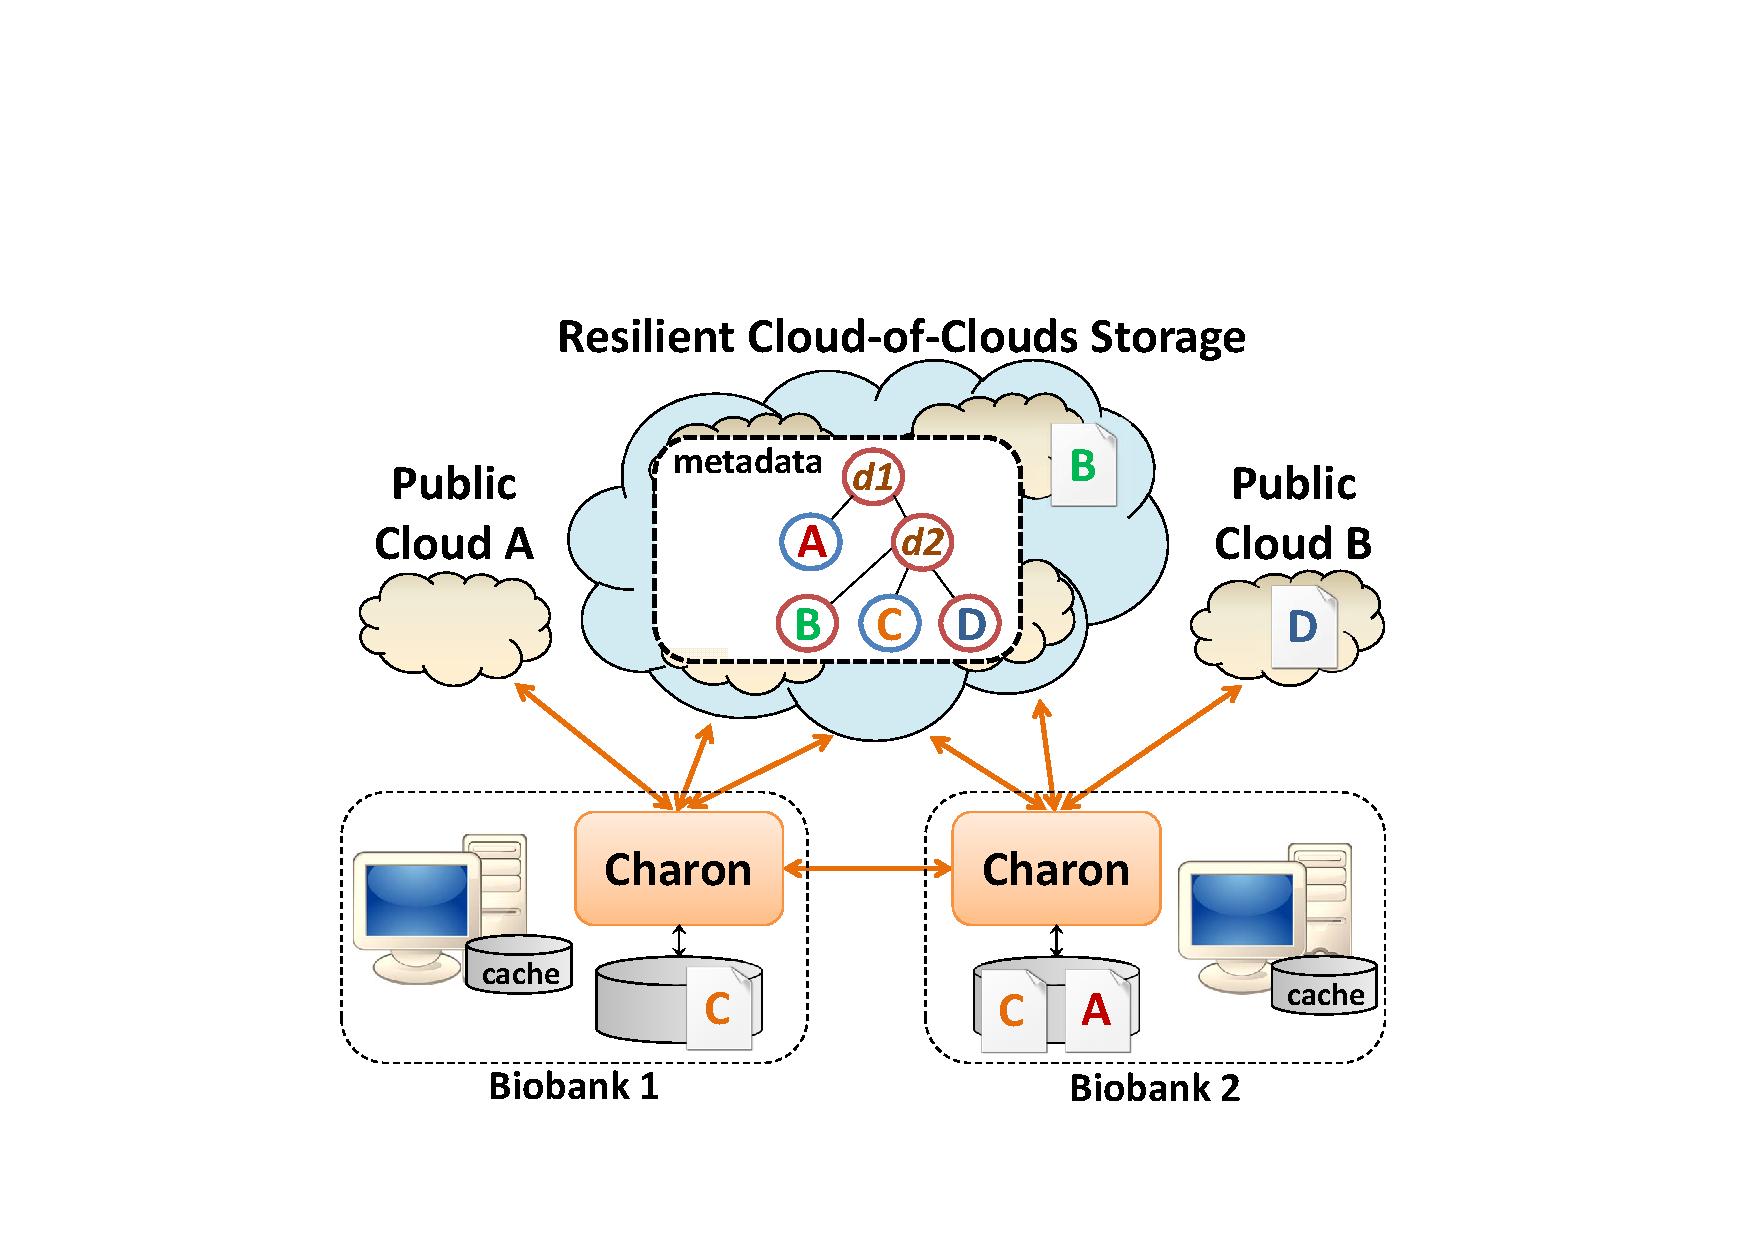
\includegraphics[width=0.6\columnwidth]{./imgs/charon_arch.pdf}
 % charon_arch.pdf: 0x0 pixel, 300dpi, 0.00x0.00 cm, bb=
\caption{\small \textsc{Charon} overview.}
\label{fig:charon}
\end{figure}
%\vskip-8pt

Two distinguishing features of \textsc{Charon} are its \emph{serverless design} and its \emph{efficient management of large files}.
The former means that no client-managed server is required in the cloud for \textsc{Charon}, which incurs in reduced maintenance costs.
The latter is achieved by employing state-of-the-art techniques for data management such as: working with data blocks instead of whole files, prefetching data blocks, multi-level cache, data compression, and background writes.
